% This is the Reed College LaTeX thesis template. Most of the work
% for the document class was done by Sam Noble (SN), as well as this
% template. Later comments etc. by Ben Salzberg (BTS). Additional
% restructuring and APA support by Jess Youngberg (JY).
% Your comments and suggestions are more than welcome; please email
% them to cus@reed.edu
%
% See https://www.reed.edu/cis/help/LaTeX/index.html for help. There are a
% great bunch of help pages there, with notes on
% getting started, bibtex, etc. Go there and read it if you're not
% already familiar with LaTeX.
%
% Any line that starts with a percent symbol is a comment.
% They won't show up in the document, and are useful for notes
% to yourself and explaining commands.
% Commenting also removes a line from the document;
% very handy for troubleshooting problems. -BTS


%%%%%%%%%%%%%%
%% Preamble %%
%%%%%%%%%%%%%%
% \documentclass{<something>} must begin each LaTeX document
\documentclass{sop_class}[overrideChapters] %modified from UF's 2019 Template --ANF
%Packages are extensions to the basic LaTeX functions. Whatever you want to
%typeset, there is probably a package out there for it. Chemistry (chemtex),
%screenplays, you name it. Check out CTAN to see: https://www.ctan.org/ Also,
%Rmarkdown can read LaTex commands in Rmd files, so long as the output is a pdf,
%because pdfs are rendered by Rmarkdown via LaTex
%%
\usepackage{siunitx}
\usepackage[artemisia]{textgreek}
\usepackage[section]{placeins}
\usepackage{pdfpages}
\usepackage{calc}
\usepackage{rotating}

% Syntax highlighting #22

% So, this code uses your CSL file to decide how to format your citations
% You may need to edit your CSL if the editorial office doesn't like it
% From {rticles}
\newlength{\csllabelwidth}
\setlength{\csllabelwidth}{3em}
\newlength{\cslhangindent}
\setlength{\cslhangindent}{1.5em}
% for Pandoc 2.8 to 2.10.1
\newenvironment{cslreferences}%
  {}%
  {\par}
% For Pandoc 2.11+
% As noted by @mirh [2] is needed instead of [3] for 2.12
\newenvironment{CSLReferences}[2] % #1 hanging-ident, #2 entry spacing
 {% don't indent paragraphs
  \setlength{\parindent}{0pt}
  % turn on hanging indent if param 1 is 1
  \ifodd #1 \everypar{\setlength{\hangindent}{\cslhangindent}}\ignorespaces\fi
  % set entry spacing
  \ifnum #2 > 0
  \setlength{\parskip}{#2\baselineskip}
  \fi
 }%
 {}
\usepackage{calc} % for calculating minipage widths
\newcommand{\CSLBlock}[1]{#1\hfill\break}
\newcommand{\CSLLeftMargin}[1]{\parbox[t]{\csllabelwidth}{#1}}
\newcommand{\CSLRightInline}[1]{\parbox[t]{\linewidth - \csllabelwidth}{#1}}
\newcommand{\CSLIndent}[1]{\hspace{\cslhangindent}#1}

\providecommand{\tightlist}{%
  \setlength{\itemsep}{0pt}\setlength{\parskip}{0pt}}
% % Added by CII (Thanks, Hadley!)
% % Use ref for internal links
\renewcommand{\hyperref}[2][???]{\autoref{#1}}
\def\chapterautorefname{Chapter}
\def\sectionautorefname{Section}
\def\subsectionautorefname{Subsection}
% End of CII addition

%%%%%%%%%%%%%%%%%%%%%%%%%%%%%%%%%
% BEGIN DOCUMENT                %
%%%%%%%%%%%%%%%%%%%%%%%%%%%%%%%%%
\begin{document}

%%%%%%%%%%%%%%%%%%%%%%%%%%%%%%%%%
% TITLE PAGE                    %
%%%%%%%%%%%%%%%%%%%%%%%%%%%%%%%%%

\docBodyfalse
\begin{center}
    \thispagestyle{empty}%
      \vspace*{-0.4in}\realSingleSpace{DETECTION OF TWO MITE-PLANT-VIRUS PATHOSYSTEMS IN FLORIDA, INCLUDING CHEMICAL ECOLOGY OF \emph{Amblyseius swirskii} AND INDUCTION OF SYSTEMIC ACQUIRED RESISTANCE ON ROSES}%
        \vfill%
        By \\*[\baselineskip]%
        \MakeUppercase{Austin N Fife}%
        \vfill%
        % A \MakeUppercase{} PRESENTED TO THE GRADUATE SCHOOL \\%
        % OF THE UNIVERSITY OF FLORIDA IN PARTIAL FULFILLMENT \\%
        % OF THE REQUIREMENTS FOR THE DEGREE OF \\%
        % \MakeUppercase{} \\*[\baselineskip]%
        % UNIVERSITY OF FLORIDA \\*[\baselineskip]%
        {2021}%
\end{center}
\newpage

%%%%%%%%%%%%%%%%%%%%%%%%%%%%%%%%%
% COPYRIGHT PAGE                %
%%%%%%%%%%%%%%%%%%%%%%%%%%%%%%%%%

\newpage
  \vspace*{\fill}
    \begin{center}
        \textcopyright{} {2021} {Austin N Fife}
    \end{center}
  \vspace*{\fill}
\newpage

\setcounter{secnumdepth}{-1}     % We don't want chapter numbers until later,
                                 % So let's kill off the table of contents depth detector until we want to start counting.
                                 

%%%%%%%%%%%%%%%%%%%%%%%%%%%%%%%%%
% TABLE OF CONTENTS             %
%%%%%%%%%%%%%%%%%%%%%%%%%%%%%%%%%

\realSingleSpace
  \tableofcontents % Table of Contents comes fourth.


%%%%%%%%%%%%%%%%%%%%%%%%%%%%%%%%%
% LIST OF TABLES                %
%%%%%%%%%%%%%%%%%%%%%%%%%%%%%%%%%

\listoftables  % List of tables comes next, if you have one.
  \addcontentsline{toc}{chapter}{LIST OF TABLES}


%%%%%%%%%%%%%%%%%%%%%%%%%%%%%%%%%
% LIST OF FIGURES               %
%%%%%%%%%%%%%%%%%%%%%%%%%%%%%%%%%

\listoffigures % List of figures comes next, if you have one.
  \addcontentsline{toc}{chapter}{LIST OF FIGURES}


%%%%%%%%%%%%%%%%%%%%%%%%%%%%%%%%%
% CHAPTERS                      %
%%%%%%%%%%%%%%%%%%%%%%%%%%%%%%%%%

    {\hypertarget{cage-set-up-and-maintenance}{%
\chapter{CAGE SET UP AND MAINTENANCE}\label{cage-set-up-and-maintenance}}

beans
\begin{figure}

{\centering 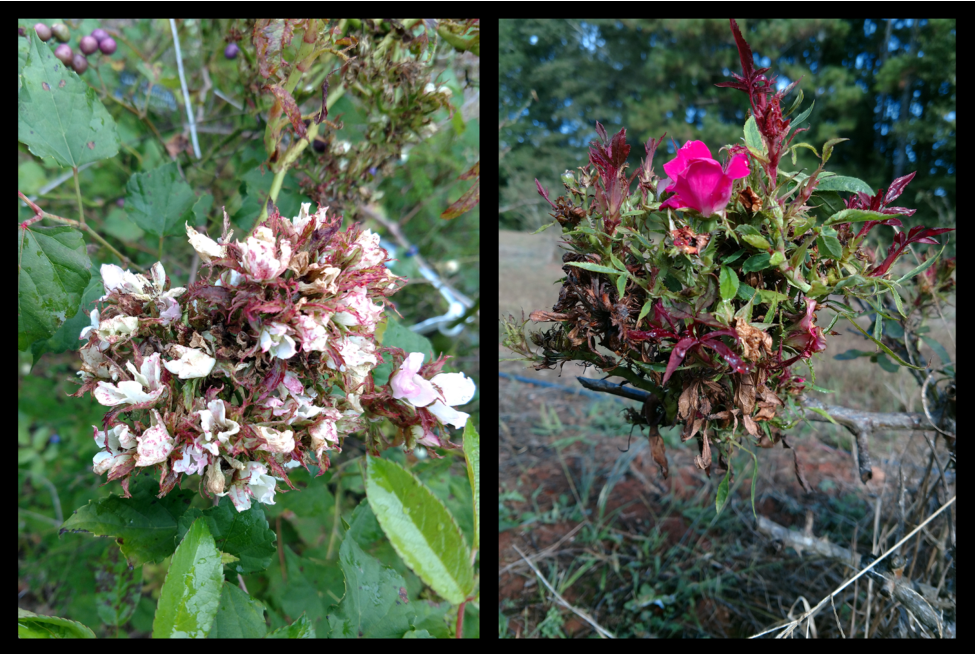
\includegraphics[width=1\linewidth]{sop_diaprepes_dundee_files/figure-latex/rrv-symptoms-1} 

}

\caption[Typical symptoms of Rose Rosette Disease (RRD), caused by \textit{Rose rosette emaravirus}]{Typical symptoms of Rose Rosette Disease (RRD), caused by \textit{Rose rosette emaravirus}: clusters of deformed flowers known as rosettes/witches' brooms, increased thorniness, elongated shoots, reddened leaves and stems. RRD ultimately kills the rose host.}\label{fig:rrv-symptoms}
\end{figure}
\docBodyfalse
\setcounter{secnumdepth}{-1}

\realSingleSpace

\hypertarget{references}{%
\chapter*{REFERENCES}\label{references}}
\addcontentsline{toc}{chapter}{REFERENCES}

\hypertarget{refs}{}
\begin{CSLReferences}{1}{1}
\leavevmode\vadjust pre{\hypertarget{ref-Ismay2021}{}}%
\textbf{Ismay, C., and N. Solomon}. \textbf{2021}. {thesisdown}: An updated {R} markdown thesis template using the bookdown package.

\leavevmode\vadjust pre{\hypertarget{ref-Xie2016}{}}%
\textbf{Xie, Y.} \textbf{2016}. Bookdown: Authoring books and technical documents with {R} markdown. Chapman; Hall/CRC, Boca Raton, Florida.

\leavevmode\vadjust pre{\hypertarget{ref-Xie2021}{}}%
\textbf{Xie, Y.} \textbf{2021}. Bookdown: Authoring books and technical documents with {R} markdown.

\end{CSLReferences}
\begin{center}\rule{0.5\linewidth}{0.5pt}\end{center}

nocite: \textbar{} \protect\hyperlink{ref-Xie2021}{Xie} (\protect\hyperlink{ref-Xie2021}{2021}), \protect\hyperlink{ref-Xie2016}{Xie} (\protect\hyperlink{ref-Xie2016}{2016}), \protect\hyperlink{ref-Ismay2021}{Ismay and Solomon} (\protect\hyperlink{ref-Ismay2021}{2021})
\ldots{}

\docBodyfalse

--\textgreater{}
--\textgreater{}
--\textgreater{}
--\textgreater{}
--\textgreater{}
--\textgreater{}

\hypertarget{appendix}{%
\chapter*{APPENDIX}\label{appendix}}
\addcontentsline{toc}{chapter}{APPENDIX}

beans

\let\chapter\appendixChapter

\titleformat{\appendixChapter }[hang]{\uppercase}{}{0pt}{\centering\realSingleSpace\ifdocBody CHAPTER \thechapter \\[-5pt] \fi}\raggedright\doublespacing}                       % This imports the body chapters included in the _bookdown.yml file,
% you can add as many chapters as you need

%%%%%%%%%%%%%%%%%%%%%%%%%%%%%%%%%
% LIST OF REFERENCES            %
%%%%%%%%%%%%%%%%%%%%%%%%%%%%%%%%%

% provided by file 98-references.Rmd

%%%%%%%%%%%%%%%%%%%%%%%%%%%%%%%%%
% APPENDICES                    %
%%%%%%%%%%%%%%%%%%%%%%%%%%%%%%%%%

% If you have multiple appendices, add them as new chapters in the 99-appendix.Rmd file

\end{document}
%%%%%%%%%%%%%%%%%%%%%%%%%%%%%%%%%
% END DOCUMENT                  %
%%%%%%%%%%%%%%%%%%%%%%%%%%%%%%%%%
